\documentclass[fleqn]{article}
\usepackage[utf8]{inputenc}
\usepackage{polski}
\usepackage{amsmath, bm}
\usepackage{titlesec}
\usepackage{graphicx}
\usepackage{caption}
\usepackage{subcaption}
\usepackage[margin= 2.8cm]{geometry}

\title{Metody interpolacji}
\author{Piotr Pesta, 184531}
\date{Maj 2022}
\setlength{\parindent}{20pt}

\graphicspath{{./Plots/}}


\begin{document}
\titlelabel{\thetitle.\quad}
\maketitle


\section{Wstęp}
    Celem projektu było zaimplementowanie dwóch metod interpolacji: metody Lagrange'a oraz funkcji skelejancyh.
    W reazlizacji zadania skorzystałem z biblioteki matplotlib do rysowania wykresów oraz modułu os do pobierania informacji o plikach w folderze.

\section{Ogólne założenia}
    Interpolacja pozwala na wyznaczenie funkjci na podstawie pewnej liczby punktów, które do niej należą. W metodach, takich jak metoda wielomianowa i
    metoda Lagrange'a, korzystamy z właśności, że n+1 punktów pozwala nam jednoznacznie wyznaczyć wielomian n-tego stopnia przechodzą przez te
    punkty. Funkcja będąca wynikiem interpolacji będzie zatem wielomianem - co niekoniecznie musi być zgodne z właściwościami oryginalnej funkcji.

    \noindent Główną wadą metod interpolacji przy użyciu wielomianów jest efekt Rungego, który można zaobserwować przy interpolacji wielomianami wysokiego stopnia.
    Powoduje on oscylacje na krańcach przedziału interpolacji. Pojawia się więc problem: mało punktów, mała dokładność - dużo punktów, efekt Rungego, jak zatem dobrać liczbę węzłów interpolacji?
    Rozwiązaniem tego problemu jest interpolacja lokalana wielomianami niskiego stopnia, co pozwala uzyskać dużą dokładność i uniknąć efektu Rungego.

    \noindent Interpolacje w taki właśnie sposób realizuje metoda funkcji sklejanych - każdy przedział jest interpolowany wielomianem 3 stopnia. 
    Wymaga ona jednak rozwiązania układu rówań liniowych, co sprawia że jest bardziej kosztowna obliczeniowo i czasowo niż metody wykorzystujące 
    wielomiany.
    
    \noindent W mojej implementacji parametr n oznacza liczbę węzłów interpolacji, a co za tym idzie, funkcja interpolowana będzie w n-1 przedziłach.
    Układ rówań w metodzie funkcji sklejanych rozwiązuje metodą faktoryzacji LU z pivotinigiem, udotsępnioną przez prowadzącego na stronie kursu.
\section{Metoda Lagrange'a}
    Metoda Lagrange'a korzysta z faktu, że n+1 punktów definiuje jednoznacznie wielomian n-tego stopnia. 
    Wartość funkcji interpolującej w dowolnym punkcie x wynosi:

    
    \[ 
        F(x) = \sum_{i = 0}^{n} y_i\phi_i(x)   
   \]
   \[
        \phi_i(x) = \prod_{j=0, j \neq i}^n \frac{x - x_j}{x_i - x_j}     
   \]

    \noindent Zaletą tej metody jest fakt, że nie trzeba tworzyć i rozwiązywać układu równań, co może być kosztowne obliczeniowo.
    Największą jej wadą jest natomiast efekt Rungego, który pojawia się przy interpolacji równo-odległych punktów przy użyciu wielomianów
    wysokiego stopnia. Zaczyna być widoczny dla n = 10, a wraz ze wzrostem n oscylacje stają się coraz większe.
    \newpage
    \begin{figure}[h]
        \centering
        \begin{subfigure}{.5\textwidth}
          \centering
          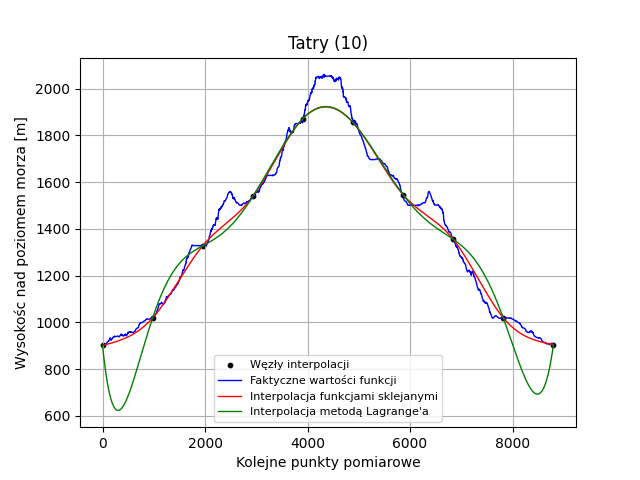
\includegraphics[width=\linewidth]{plot_10_points_Tatry.png}
          \caption{Przykład dla n = 10}
          \label{fig:sub1}
        \end{subfigure}%
        \begin{subfigure}{.5\textwidth}
          \centering
          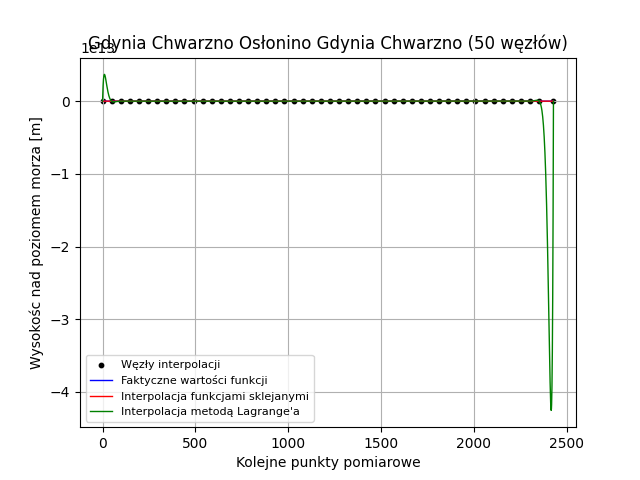
\includegraphics[width=\linewidth]{efektRungego.png}
          \caption{Przykład dla n = 50}
          \label{fig:sub2}
        \end{subfigure}
        \caption{Efekt Rungego}
        \label{fig:test}
    \end{figure}

    \noindent Jak widać na powyższych wykresach, metoda Lagrange'a dla dużych n daje bardzo złe rezultaty, a dla mniejszych n, dokładność interpolacji może nie być zadowoalająca.
    Sprawia to, że metoda ta jest średnio przydatna, szczególnie jeżeli zależy nam na sotsunkowo dokładnym wyznaczeniu funkcji interpolującej.

\newpage
\section{Interpolacja funkcjami sklejanymi}
    W metodzie interpolacji funckjami sklejanymi stosujemy interpolacje lokalną - dla każdego przedziału stosujemy interpolacje wielomianem niskiego stopnia.
    Pozwala to na uzyskanie dobrej dokładności przy jednoczesnym braku efektu Rungego.

    \noindent To rozwiązanie jest jednak bardziej kosztowne obliczeniowo, ze względu na koniczeność ułożenia i rozwiązania ukłądu równań liniowych. 
    Ma to na celu wyznacznenie współczynników n wielomianów (po 1 na przedział interpolacji) 3 stopnia. Układ ten będzie zatem zawierał 4n równań i 4n niewiadomych

    \noindent Konstrukcja układu:
    \begin{itemize}
        \item $S_i(x_i) = f(x_i)$ - ustalona wartość w węzłach interpolacji
        \item $S_i(x_{i+1}) = f(x_{i+1})$ - ciągłość funckji w węzłach
        \item $S_i'(x_{i+1}) = S_{i+1}'(x_{i+1})$ - ciągłość pierwszej pochodnej w węzłach
        \item $S_i''(x_{i+1}) = S_{i+1}''(x_{i+1})$ - ciągłość drugiej pochodnej w węzłach
        \item $S_0''(x_0) = 0, \; S_{n-1}''(x_n) = 0 $ - zerowanie drugiej pochodnej w węzłach granicznych
    \end{itemize}

    \noindent Postać funkcji S(x):
    \begin{itemize}
        \item $S_i(x) = a_i + b_i(x - x_i) + c_i(x - x_i)^2 + d_i(x-x_i)^3 $
        \item $S_i'(x) = b_i + 2c_i(x - x_i) + 3d_i(x - x_i)^2 $
        \item $S_i''(x) = 2c_i + 6d_i(x-x_i) $
    \end{itemize}

    \noindent Po podstawienu wartości powstaje następujący układ równań $(h = x_{i+1} - x_i)$

    \[
    \begin{cases}
        a_0 = f(x_0)\\
        a_0 + b_0h + c_0h^2 + d_0h^3 = f(x_1)\\
        b_0 + 2c_0h + 3d_0h^2 = b_1\\
        2c_0 + 6d_0h = 2c_1\\
        \vdots \\
        a_{n-1} = f(x_{n-1})\\
        a_{n-1} + b_{n-1}h + c_{n-1}h^2 + d_{n-1}h^3 = f(x_{n-1})\\
        b_{n-1} + 2c_{n-1}h + 3d_{n-1}h^2 = b_{n}\\
        2c_{n-1} + 6d_{n-1}h = 2c_{n-1}\\
        a_n = f(x_n) \\
        a_n + b_nh + c_nh^2 + d_nh^3 = f(x_{n+1})\\
        c_0 = 0 \\
        2c_n + 6d_nh = 0
    \end{cases}    
    \]

    \noindent Układ ten zbudowany jest z n-1 czwórek rówań dla każdego przedziału, dwóch równań dla ostatniego przedziału
    oraz dwóch rówanań dla skrajnych punktów.

    \noindent Po jego rozwiazaniu otrzymamy współczyniki wielomianów interpolujących wszystkie przedziały. W celu ich obliczenia dokonałem
    zapisu powyższego układu w postaci macierzowej, a następnie do jego rozwiązania wykorzystałem metodę faktoryzacji LU z projektu nr 2 z dodanym pivotingiem.

    \newpage

    \noindent Porównanie interpolacji funkcjami sklejanymi i metodą Lagrange'a (na wykresach dla większych n nie umieściłem wyniku interpolacji
    Lagrange'a, ponieważ występujący efekt Rungego znacznie pogorszył czytelność wykresu)
    \begin{figure}[h]
        \centering
        \begin{minipage}{.33\textwidth}
            \centering
            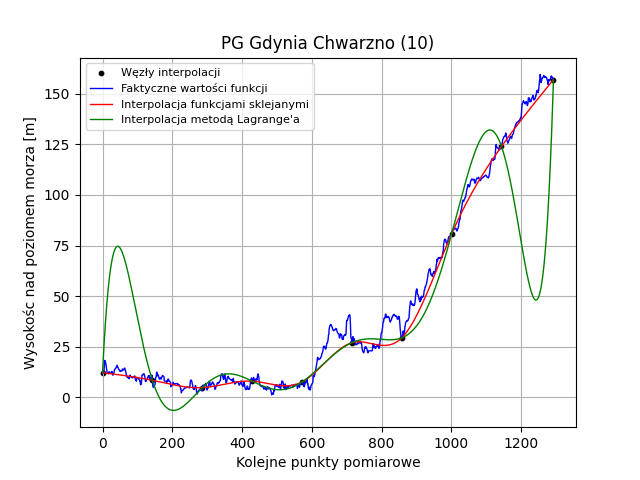
\includegraphics[width=\linewidth]{plot_10_points_PG_Gdynia_Chwarzno.png}
            \label{fig:sub1}
        \end{minipage}%
        \begin{minipage}{.33\textwidth}
          \centering
          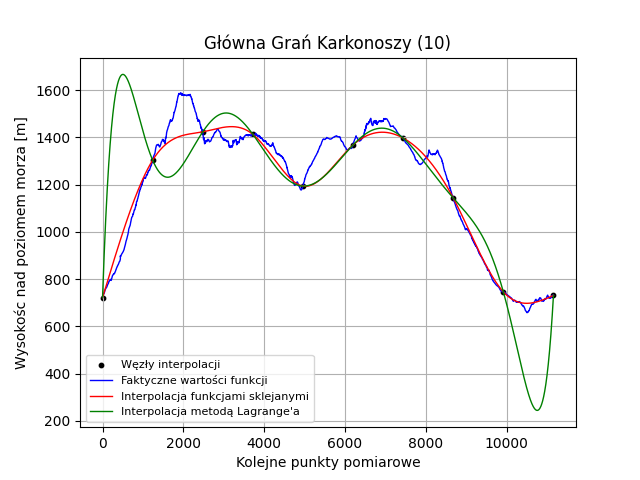
\includegraphics[width=\linewidth]{plot_10_points_Główna_Grań_Karkonoszy.png}
          \label{fig:sub2}
        \end{minipage}%
        \begin{minipage}{.33\textwidth}
          \centering
          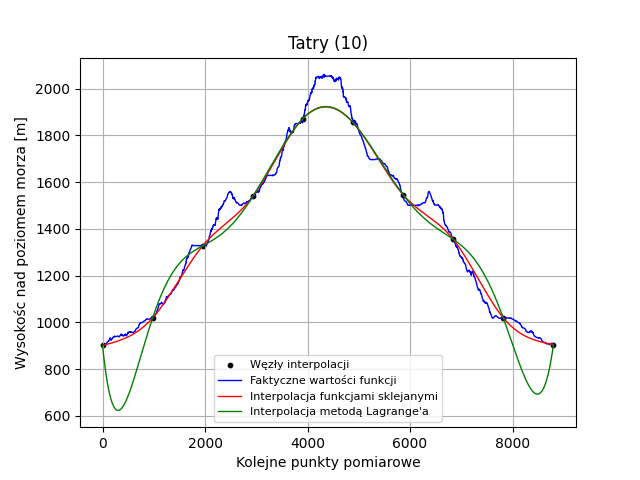
\includegraphics[width=\linewidth]{plot_10_points_Tatry.png}
          \label{fig:sub3}
        \end{minipage}
        \caption{Przykłady dla n = 10}
        \label{fig:test}
    \end{figure}
    \begin{figure}[h]
        \centering
        \begin{minipage}{.33\textwidth}
            \centering
            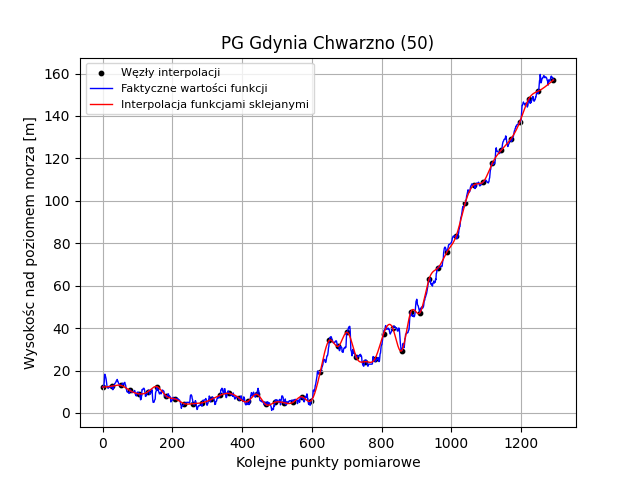
\includegraphics[width=\linewidth]{plot_50_points_PG_Gdynia_Chwarzno.png}
            \label{fig:sub1}
        \end{minipage}%
        \begin{minipage}{.33\textwidth}
          \centering
          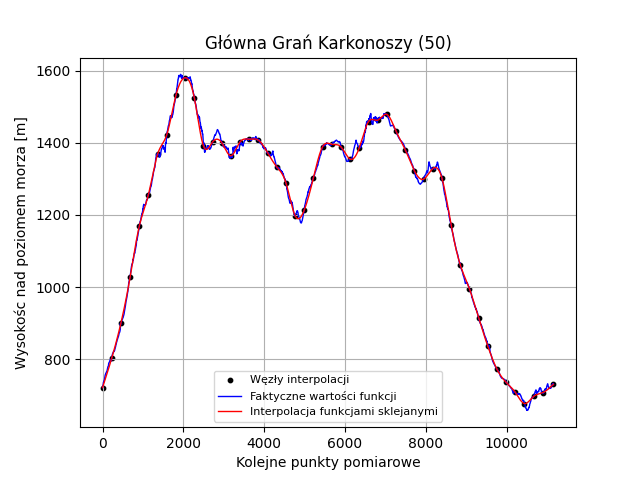
\includegraphics[width=\linewidth]{plot_50_points_Główna_Grań_Karkonoszy.png}
          \label{fig:sub2}
        \end{minipage}%
        \begin{minipage}{.33\textwidth}
          \centering
          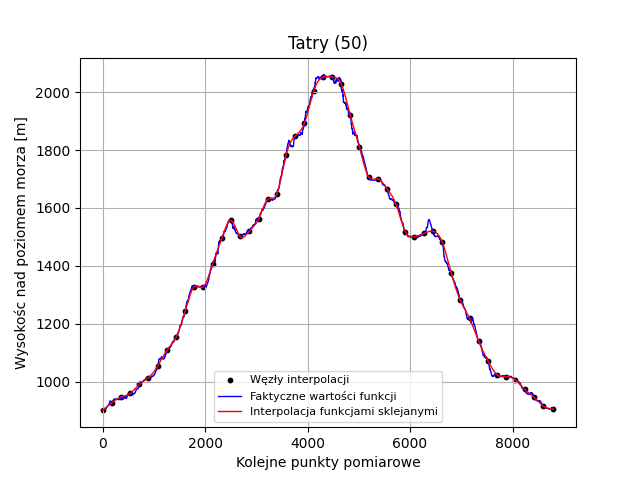
\includegraphics[width=\linewidth]{plot_50_points_Tatry.png}
          \label{fig:sub3}
        \end{minipage}
        \caption{Przykłady dla n = 50}
        \label{fig:test}
    \end{figure}
    \begin{figure}[h]
        \centering
        \begin{minipage}{.33\textwidth}
            \centering
            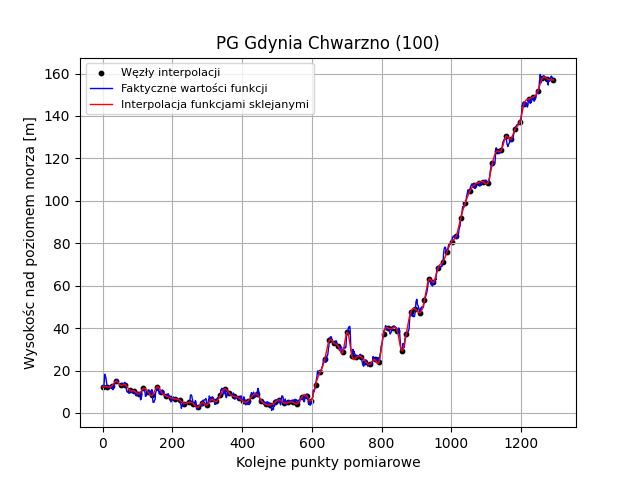
\includegraphics[width=\linewidth]{plot_100_points_PG_Gdynia_Chwarzno.png}
            \label{fig:sub1}
        \end{minipage}%
        \begin{minipage}{.33\textwidth}
          \centering
          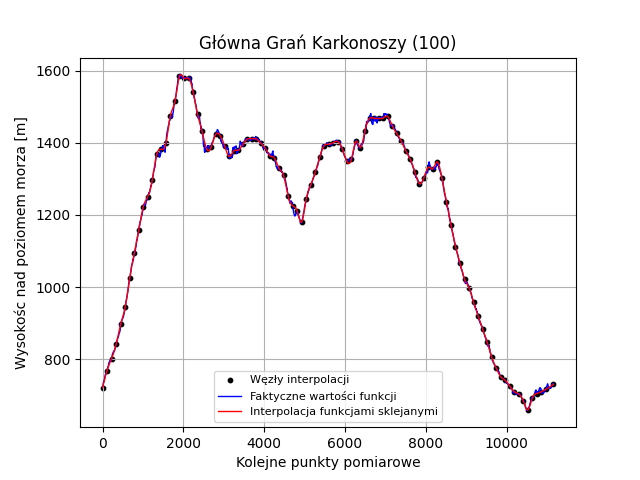
\includegraphics[width=\linewidth]{plot_100_points_Główna_Grań_Karkonoszy.png}
          \label{fig:sub2}
        \end{minipage}%
        \begin{minipage}{.33\textwidth}
          \centering
          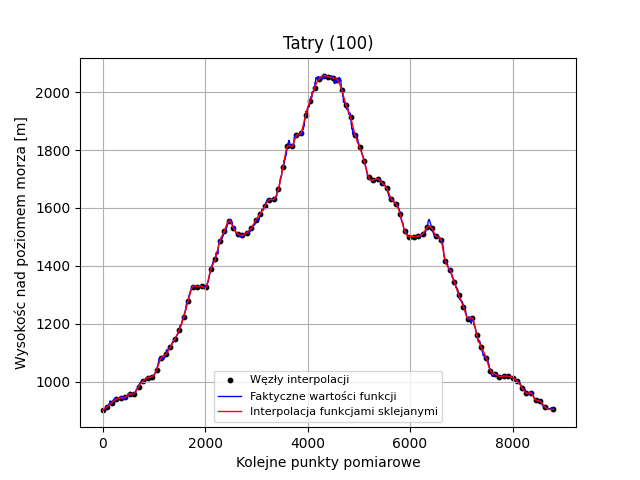
\includegraphics[width=\linewidth]{plot_100_points_Tatry.png}
          \label{fig:sub3}
        \end{minipage}
        \caption{Przykłady dla n = 100}
        \label{fig:test}
    \end{figure}

    Jak widać na wykresach, interpolacja splineami daje dobre wyniki dla n = 10, a dla wysokich n otrzymujemy prawie dokładny wykres funkcji.
\newpage
\section{Analiza wyników}
\subsection{Wpływ liczby punktów węzłowych na wynik}
    Analizując wyniki obu metod, możemy zauważyć, że im więcej punktów tym dokładniejsza interpolacja. 
    Metoda Lagrang'e nie daje zadowalających rezulatatów dla większych ilości punktów pomiarowych,
    jest to spowodowane występowaniem efektu Rungego. Większa ilość punktów nie jest też bez znaczenia dla metody interpolacji
    funkcjami sklejanymi. Wymaga ona rozwiązania układu równań, a koszt tej operacji jest wprost proporcjonalny do liczby zmiennych (faktoryzacja LU - $O(n^3)$).
\subsection{Korekcja błędów}
    Zależnie od umiejscowienia węzłów interpolacji, algorytmy mogą zniwelować błędy GPS. Widać to na poniższym przykładzie.
    \begin{figure}[h]
      \begin{minipage}{.5\textwidth}
        \centering
        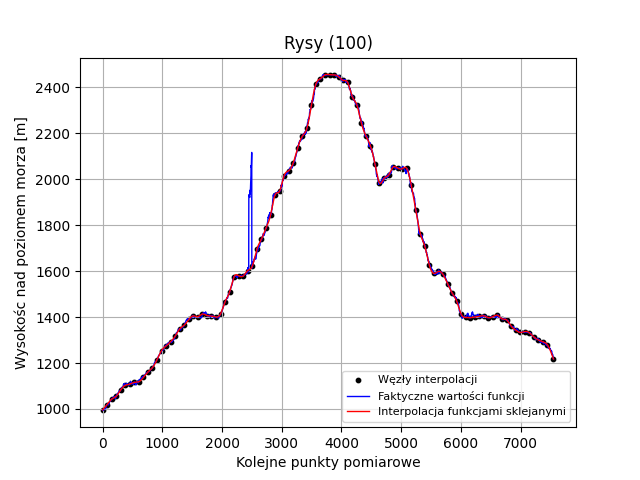
\includegraphics[width=\linewidth]{plot_100_points_Rysy.png}
        \captionof{figure}{Błąd został skorygowany}
        \label{fig:test1}
      \end{minipage}%
      \begin{minipage}{.5\textwidth}
        \centering
        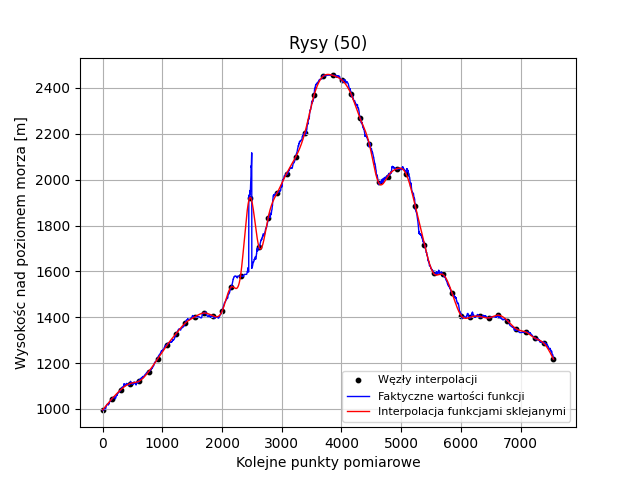
\includegraphics[width=\linewidth]{plot_50_points_Rysy.png}
        \captionof{figure}{Błąd widoczny na wyniku interpolacji}
        \label{fig:test2}
      \end{minipage}
    \end{figure}

    \noindent Jak widać zdolność do korekcji zależy jedynie od doboru punktów, a nie od gęstości ich rozmieszczenia.
    Na powyższym przykładzie widać, że dla teoretycznie mniej dokładnej interpolacji w 50 punktach błąd jest widoczny,
    a dla 100 węzłów, punkty zostały rozmieszczone w taki sposób, że błąd ma znaczący wpływ na wynik interpolacji.
  \newpage
  \subsection{Wpływ charakteru trasy na wyniki}
    Przy interpolacji z większą ilością pnktów węzłowych, charakter trasy nie wpływa na wyniki algorytmu (mówimy o algorytmie funkcji sklejanych).
    Dla n równego 5 oraz 10, algorytm daje zadowalające przybliżenie dla tras mało dynamicznych, a w przypadku tras o dużych i szybkich różnicach wysokości,
    niektóre ekstrema lokalne zostają pominięte. Analizujemy wykres interpolacji uzyskany w metodzie funkcji sklejanych, ponieważ w jej przypadku
    nie występuje efekt Rungego.
    \begin{figure}[h]
      \begin{minipage}{.5\textwidth}
        \centering
        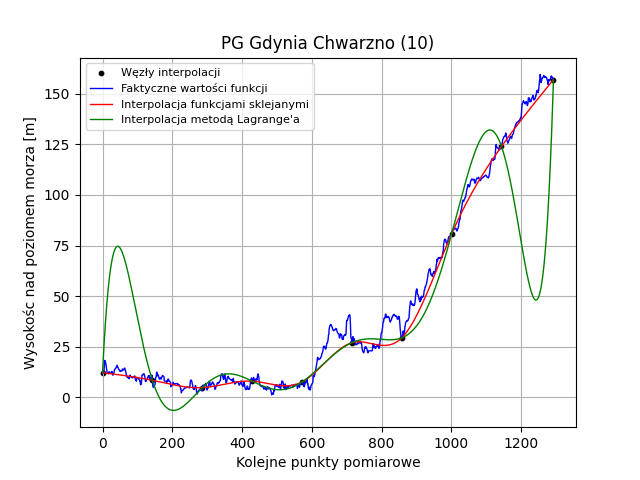
\includegraphics[width=\linewidth]{plot_10_points_PG_Gdynia_Chwarzno.png}
        \captionof{figure}{Trasa mało dynamiczna - dobry wynik dla małej liczby punktów interpolacji}
        \label{fig:test1}
      \end{minipage}%
      \begin{minipage}{.5\textwidth}
        \centering
        \includegraphics[width=\linewidth]{plot_10_points_Gdynia_Chwarzno_Osłonino_Gdynia_Chwarzno.png}
        \captionof{figure}{Trasa bardziej dynamiczna - część ekstremów została pominięta}
        \label{fig:test2}
      \end{minipage}
    \end{figure}
\end{document}